% !TeX root = ../main.tex
% Add the above to each chapter to make compiling the PDF easier in some editors.
% comment out multiple lines with ctrl + '/'


\chapter{Related work}\label{chapter:Related_work_tracking}

In modern dynamic vision, tracking is encountered, directly or implicitly, in different problem formulations related to video understanding. For example, the tasks of \acrlong{MOTS} (\acrshort{MOTS}) \parencite{mots20}, \acrlong{VIS} (\acrshort{VIS}) \parencite{Yang2019vis}, \acrlong{VPS} (\acrshort{VPS}) \parencite{kim2020vps} and \acrlong{VOS} (\acrshort{VOS}) \parencite{davis} are closely connected and involve tracking as part of their objectives. All these problems tackle object detection in videos, but present differences in how the background class is treated or whether multiple instances of the same semantic class are encountered in the data.
These distinctions in the problem formulation and objectives result in differences in the approaches and evaluation metrics introduced in the literature. However, in many cases inspiration can be drawn from solutions originally proposed for different problem paradigms. \par

As already mentioned in the introduction, the main goal of this thesis is to propose a DL model that predicts temporally consistent object segmentation masks in the context of robotics. Our class-agnostic problem formulation is closer to the VOS task, that is typically tackled with semi-supervised learning approaches. However, inspiration can also be drawn to some extent by concepts encountered in VIS and MOTS. For that matter, we aim at reviewing a wide range of algorithms and concepts that are available in the literature and may be relevant for a good solution for the task at hand.\par

To simplify the review process of existing works that may be relevant for designing a robust tracker in the robotic setup, three levels of categorisation are proposed. First, a distinction is made between \textbf{online} and \textbf{offline} tracking methods. For the \textbf{online} methods, that are more relevant to the task at hand, a distinction is also made between \textbf{modular} and \textbf{end-to-end}. Finally, online modular tracker are split into two subgroups, \textbf{heuristic based} and \textbf{learning based}. A summary visualisation of the categories involved in this review is provided in \figref\ref{fig:taxonomies}. It is worth noting that \figref\ref{fig:taxonomies} does not involve all possible sub categories encountered in each group, but rather only the ones presented in this review and are most relevant to our problem. \par


\section{Taxonomies of tracking methods}\label{seq:taxonomies}

\begin{figure}
    \centering
    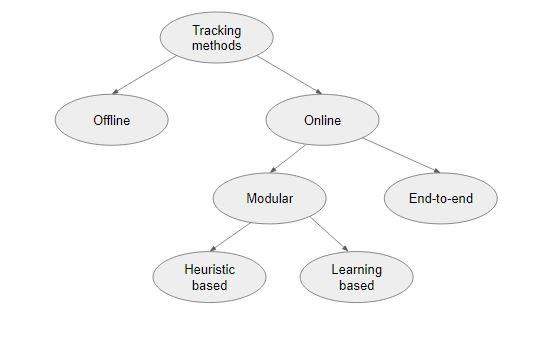
\includegraphics[]{figures/02_review/taxonomies.jpg}
    \caption{Proposed taxonomies for tracking methods}
    \label{fig:taxonomies}
\end{figure} 

The first intuitive way to categorise tracking approaches is between \textbf{online} and \textbf{offline} approaches. \textbf{Offline} approaches typically receive as input a batch of frames which is available in advance. Offline methods typically demonstrate superior performance compared to online methods, since optimization is taking place in both directions of time, as the model has access to data from both past and future frames. Offline methods though more powerful can only be used to analyse prerecorded video sequences and hence are not directly applicable in real time applications such as robotic tracking. In the case of \textbf{online} approaches on the other hand the input frames are handled in a sequential manner \parencite{reviewTracking}. This implies that the model can only learn from one or multiple past frames stored in a memory module. Therefore, online approaches are the only viable alternative for real-life applications like autonomous driving or robotic manipulation. \par
% \comMD{I'd explain this a bit more in detail. What does step-wise manner mean? Perhaps you start with offline tracking and then transfer to online by mentioning what makes the online one more challenging etc.? }

    
% \comWB{you could also move the respective paragraphs to the respective sections (2.1.1/2), and here only say e.g. that in online settings no future frames are available?    

% \comMD{I am missing the benefits and drawbacks of both groups here. E.g., why would I consider offline approaches?}
% \comWB{+1. I think you could also mention fine-tuning / optimization across frames for offline methods (hodor does that for example; they could online optimize with their full forward/backward processing just given a single annoated frame). online this isn't possible - not just because the compute is too small, but also because you can't look into the future.}
% \comST{I think this is addressed inside the offline methods section, where i compare STMs with their offline counterpart}
Online methods can be further split into two groups, \textbf{end-to-end} and \textbf{modular}, depending on how tracking is performed. In general, tracking can be seen as a combination of two subtasks: single shot object detection/localisation ignoring the aspect of time and time consistent object detection with id assignment \parencite{hota}. End-to-end methods, typically learning based, perform detection and tracking jointly with a single module. Modular methods on the other hand, be it heuristic based or learning based, involve separate modalities in the tracking pipeline. For example, heuristic based modular methods tackle the two subtasks independently with two separate modules, one for single shot detection and one for detection association (tracking). Learning based modular trackers on the other hand typically require some initialisation for the tracking process. Hence, they feature a DL network that produces temporally consistent detections, but the inference process is initialised by a separate single shot object detector.

% The two models can be both \textbf{learning based}, or in the more traditional variant, the detector can be learning based and the tracker \textbf{heuristic based}. Either way, in the modular setup the detector can be trained separately and can be treated as a separate module from the tracker. End-to-end methods on the other hand perform detection and tracking jointly with a single module. Modular methods on the other hand require  They typically comprise of deep learning models trained jointly for the combined task in a holistic fashion. Since end-to-end models have a more complex optimization objective, they tend to be harder to train compared to their modular counterparts in the online setup. \par

In the following sections, an overview of \gls{SOTA} methods belonging to each of the proposed categories is provided. Since the goal is to propose a solution for robotic tracking, more focus is posed on online methods and their subcategories. However, even a short overview of each subcategory can help understand trends in current research and draw inspiration for a solution that involves desired attributes. \par

% Modularity is also a desirable attribute, but end-to-end methods can also help us guide us towards the optimal solution on a more high level. Finally, learning based modular approaches are more attractive, since we'd like to leverage the power of deep learning to propose a more robust and efficient solution for our problem.
%In the following sections,

% \comMD{again :) I would add some more attributes of the methods as well as the benefits and drawbacks}
% In general,


\section{Offline tracking methods}
Most SOTA methods in offline tracking are transformer based. Notable examples of offline tracking methods that demonstrate superior performance on YouTube-VIS \parencite{Yang2019vis} are VisTR\parencite{visTR} and its improvements DeVIS \parencite{devis} and SeqFormer \parencite{seqformer}. All three methods extend a transformer based object detection algorithm, either DETR \parencite{DETR} in the case of \parencite{visTR} or deformable DETR \parencite{zhu2020deformable} in the cases of \parencite{devis} and \parencite{seqformer} in the temporal domain. As expected, computing spatio-temporal attention is very computationally expensive, so \parencite{devis} and \parencite{seqformer} introduce improvements like the use of deformable attention in \parencite{devis} or a more efficient way to handle object queries on a video level in \parencite{segformer}. The computational complexity of attention mechanism is a problem that both online and offline methods suffer from. \par

 As already mentioned in \autoref{seq:taxonomies}, a significant advantage of offline tracking methods is that optimisation takes place in both directions of time during training. For example, in \parencite{park2022per} the authors present an offline version of STMs \parencite{stm} by conducting both memory update and mask prediction on a clip (set of consecutive frames) instead of frame level achieving superior performance to STMs. In practice  these algorithms can only serve loosely as source of inspiration for the solution to be designed. Realistically, learning from multiple frames in a batched fashion is not applicable in tracking for autonomous systems.\par

\section{Online tracking methods}
In the case of online tracking, more versatility is encountered among the methods that demonstrate SOTA performance.
Examples of online approaches in tracking span from the simple but powerful SORT\parencite{sort} and DeepSORT \parencite{deepsort} to the transformer-based Trackformer \parencite{meinhardt2021trackformer} and IDOL \parencite{IDOL}. However, the most powerful online methods achieving comparable performance with offline methods on challenges like YouTube-VIS \parencite{Yang2019vis} and MOTS20 \parencite{mots20} are DL based.\par


\subsection{Heuristic based Modular Online methods}

There is a wide range of heuristic based modular online tracking methods that decouple the detection from the tracking process. 
% In some cases, tracking is approached as a simple post-processing step of the detections that does not involve learning. \comMD{I would not call it "simple post-processing" since it is the main part of detections +tracking, or?}
% In the semi-supervised setup, however, the tracker can be a separate neural network that is 'guided' by the detector during inference with a certain frequency (fps). \comMD{fps are normally introduced as frames per second and not as the frequency which is normally Hz}
% \comMD{not sure what you want to say with the last two sentences}
% \par 
However, most heuristic based modular trackers involve some sort of motion or appearance assumption. For example, in the case of Kalman Filters \parencite{kalmanfilter} a linear motion assumption is made. Another common modular approach may involve some sort of matching based on appearance similarity like the \gls{IoU} association baseline used in \parencite{step}. In IoU association, a unique track id is initialised for each detected object in the first frame and this id is propagated in the next frames with a linear sum assignment algorithm like the Hungarian method based on IoU overlap scores between detections. 
Other examples of modular methods may involve a Markov decision process like the method proposed in \parencite{mdp} or some sort of optical flow warping \parencite{raft} of predicted masks from $t-1$ in $t$ combined also with an IoU association/ matching step \parencite{step}.\par
A particularly interesting modular tracker is SORT \parencite{sort}, a Kalman-based tracking method with a data association step. 
SORT can be combined with any probabilistic detector, as it uses confidence scores apart from bounding boxes to estimate the position of the tracked object in the next frame. 
The method owes its popularity to its relatively high performance on the MOT challenge \parencite{mot17} despite its simplicity. 
SORT is often used as baseline for more complex learning based approaches like \cite{unicorn}, which have long outperformed heuristic based tracking in all important evaluation benchmarks.

\subsection{End-to-end Online methods}


 The term end-to-end refers to methods that entail some sort of modification or further training on the detector they build upon.
% For our enhanced INSTR use case, choosing an end-to-end approach is also more tedious and involves further training/ fine-tuning at least some layers of the model. \par
In the literature, a variety of end-to-end tracking algorithms is encountered, like the LSTM-based tracker introduced in \parencite{gordon2017re3} or the transformer-based Trackformer \parencite{meinhardt2021trackformer}.\par
One quite dominating concept in converting transformer-based detectors into end-to-end trackers is the concept of track queries. In Trackformer \parencite{meinhardt2021trackformer} the authors adjust deformable DETR \parencite{zhu2020deformable} for tracking by making use of the concept and report very good results on the MOT17 \parencite{mot17}, MOT20 \parencite{mot20} and MOTS20 challenges \parencite{mots20}. 
In \parencite{Rovis} the authors adapt the powerful MaskFormer \parencite{cheng2021maskformer} and achieve very good results on the VIS benchmarks OVIS \parencite{ovis} and UVO \parencite{uvo}. 
The notion of propagating high-level information from detections of the previous frame is not solely encountered in supervised end-to-end trackers that work in \parencite{meinhardt2021trackformer} and \parencite{Rovis}. 
In a way, the concept of 'slots' proposed in \parencite{savi} and the high-level features in \parencite{athar2022hodor} act for the model similarly to 'track' queries propagating previous information on a detection level. 
This is in contrast to information propagation performed on a feature map level from the previous frame preferred in memory-based methods like \parencite{stm} and \parencite{yang2021aot}, which is in general more computationally intensive. \par

A notable transformer-based online tracker is IDOL \parencite{IDOL}. IDOL uses contrastive learning to perform tracking by association based on appearance similarity. 
% After passing two adjacent frames through shared feature extraction layers, the decoded embeddings are led to contrastive head. 
The use of a contrastive loss enables the model to learn more discriminative embeddings for association, achieving comparable results to offline trackers.
%Another powerful online tracker is Unicorn \parencite{unicorn}. 
A less resource demanding transformer-based architecture is Unicorn \parencite{unicorn}. 
% Unicorn falls in the category of general vision models, as it attempts to address multiple different vision problems with one architecture.
In Unicorn, a matching mechanism with deformable attention is used to capture interactions between neighboring frames. Matching mechanisms as a concept are present in many works on online tracking and are very effective in propagating information from previous frames. They can be applied on a feature map level like in \parencite{stm} or on higher order descriptors (generated from the ground truth) like in \parencite{athar2022hodor}.\par

Most end-to-end methods encountered in the literature are supervised learning models designed to track many instances of the same semantic class, like cars or pedestrians. This attribute of end-to-end online methods is not compatible with our class-agnostic problem formulation. Therefore, a different category of online learning based methods is also reviewed, to help us propose a solution that better accommodates the problem's requirements.



\subsection{Learning based Modular Online methods}

An alternative to end-to-end learning based online methods, which are typically supervised, are semi-supervised tracking approaches. Unlike supervised methods, semi-supervised trackers require an initialisation in the first frame, either via the ground truth annotations for the objects to-be-tracked or via the predicted objects from another network. Hence, semi-supervised are modular by their nature, as they can be easily combined with different object detectors for initialization without further adjustment.  \par

An important semi-supervised, learning based modular online tracker is the memory based approach proposed in Space-Time Memory networks (STM)\parencite{stm}. The memory based approach in STM involves storing past encoded feature maps in a memory module. Then the stored past feature maps are utilised in learned spatio-temporal matching with the current encoded feature map to produce the current frame predictions. \par
The idea of storing extracted features from multiple past frames in a memory module to boost prediction performance on a video sequence first introduced in \parencite{stm} has been very influential for the current SOTA semi-supervised methods.
For example, AOT and its variants \parencite{yang2021aot}, \parencite{yang2021aost}, \parencite{yang2022deaot} propose a more efficient way to perform multi-object matching and segmentation. Instead of performing matching and decoding for each mask (target) in parallel, they propose an efficient way to project and associate multiple objects in the same high dimensional embedding space. On a different note, XMem  \parencite{cheng2022xmem} leverages a more elaborate memory mechanism with multiple independent memory modules, thus achieving superior performance in longer videos compared to STM and its variants.
\newpage
The concept of learned spatio-temporal matching, typically with an attention mechanism, has been very influential also for more lightweight online methods that omit the memory module and only match with information from a single past frame like \parencite{savi}, \parencite{athar2022hodor}. These methods also distinct themselves from memory based approaches since they propagate past information on a ground truth/prediction instead of feature map level. More specifically, the authors in \parencite{savi} compare a variety of different cue sources from the first frame ground truth (center of mass, bounding box, segmentation) and demonstrate that even the most naive motion cues from the first frame - such as the center of mass of detected objects suffice for successful tracking of objects in the next frames. 
On the other hand, in \parencite{athar2022hodor} the authors demonstrate that even just high-order descriptors from the first frame detection (the whole segmentation mask instead of feature maps) can help to guide the model for association consistency in upcoming frames. \par

